\documentclass[a4paper,12pt]{article}

% Этот шаблон документа разработан в 2014 году
% Данилом Фёдоровых (danil@fedorovykh.ru) 
% для использования в курсе 
% <<Документы и презентации в \LaTeX>>, записанном НИУ ВШЭ
% для Coursera.org: http://coursera.org/course/latex .
% Исходная версия шаблона --- 
% https://www.writelatex.com/coursera/latex/5.3

% В этом документе преамбула

%%% Работа с русским языком
\usepackage{cmap}					% поиск в PDF
\usepackage{hyperref}
\usepackage{mathtext} 				% русские буквы в формулах
\usepackage[T2A]{fontenc}			% кодировка
\usepackage[utf8]{inputenc}			% кодировка исходного текста
\usepackage[english, russian]{babel}	% локализация и переносы
\usepackage{indentfirst}
\frenchspacing

\DeclareSymbolFont{T2Aletters}{T2A}{cmr}{m}{it}

%\usepackage{algorithm}
%\usepackage{algpseudocode}
\usepackage[linesnumbered,ruled,vlined]{algorithm2e}
\RestyleAlgo{ruled}
\SetKwInput{KwData}{Input}
\SetKwInput{KwResult}{Output}

\usepackage{relsize}

\renewcommand{\epsilon}{\ensuremath{\varepsilon}}
\renewcommand{\phi}{\ensuremath{\varphi}}
\renewcommand{\kappa}{\ensuremath{\varkappa}}
\renewcommand{\le}{\ensuremath{\leqslant}}
\renewcommand{\leq}{\ensuremath{\leqslant}}
\renewcommand{\ge}{\ensuremath{\geqslant}}
\renewcommand{\geq}{\ensuremath{\geqslant}}
\renewcommand{\emptyset}{\varnothing}

%%% Дополнительная работа с математикой
\usepackage{amsmath,amsfonts,amssymb,amsthm,mathtools} % AMS
\usepackage{icomma} % "Умная" запятая: $0,2$ --- число, $0, 2$ --- перечисление

%% Номера формул
%\mathtoolsset{showonlyrefs=true} % Показывать номера только у тех формул, на которые есть \eqref{} в тексте.
%\usepackage{leqno} % Нумереация формул слева

%% Свои команды
\DeclareMathOperator{\sgn}{\mathop{sgn}}

%% Перенос знаков в формулах (по Львовскому)
\newcommand*{\hm}[1]{#1\nobreak\discretionary{}
{\hbox{$\mathsurround=0pt #1$}}{}}

%%% Работа с картинками
\usepackage{graphicx}  % Для вставки рисунков
\graphicspath{{images/}{images2/}}  % папки с картинками
\setlength\fboxsep{3pt} % Отступ рамки \fbox{} от рисунка
\setlength\fboxrule{1pt} % Толщина линий рамки \fbox{}
\usepackage{wrapfig} % Обтекание рисунков текстом

%%% Работа с таблицами
\usepackage{array,tabularx,tabulary,booktabs} % Дополнительная работа с таблицами
\usepackage{longtable}  % Длинные таблицы
\usepackage{multirow} % Слияние строк в таблице

%%% Теоремы
\theoremstyle{plain} % Это стиль по умолчанию, его можно не переопределять.
 
\theoremstyle{definition} % "Определение"

\theoremstyle{remark} % "Примечание"
\newtheorem*{nonum}{Решение}

\newtheoremstyle{break}%
{}%
{}%
{\itshape}%
{}%
{\bfseries}%
{}%
{\newline}
{}%
\theoremstyle{break}
\newtheorem{definition}{Определение}
\newtheorem{problem}{Задача}
\newtheorem{theorem}{Теорема}[subsection]
\newtheorem{assumption}{Предположение}[subsubsection]

%%% Программирование
\usepackage{etoolbox} % логические операторы

%%% Страница
\usepackage{extsizes} % Возможность сделать 14-й шрифт
\usepackage{geometry} % Простой способ задавать поля
	\geometry{top=25mm}
	\geometry{bottom=35mm}
	\geometry{left=35mm}
	\geometry{right=20mm}
 %
%\usepackage{fancyhdr} % Колонтитулы
% 	\pagestyle{fancy}
 	%\renewcommand{\headrulewidth}{0pt}  % Толщина линейки, отчеркивающей верхний колонтитул
% 	\lfoot{Нижний левый}
% 	\rfoot{Нижний правый}
% 	\rhead{Верхний правый}
% 	\chead{Верхний в центре}
% 	\lhead{Верхний левый}
%	\cfoot{Нижний в центре} % По умолчанию здесь номер страницы

\usepackage{setspace} % Интерлиньяж
%\onehalfspacing % Интерлиньяж 1.5
%\doublespacing % Интерлиньяж 2
%\singlespacing % Интерлиньяж 1

\usepackage{lastpage} % Узнать, сколько всего страниц в документе.

\usepackage{soul} % Модификаторы начертания

\usepackage[usenames,dvipsnames,svgnames,table,rgb]{xcolor}
\hypersetup{				% Гиперссылки
    unicode=true,           % русские буквы в раздела PDF
    pdftitle={Заголовок},   % Заголовок
    pdfauthor={Автор},      % Автор
    pdfsubject={Тема},      % Тема
    pdfcreator={Создатель}, % Создатель
    pdfproducer={Производитель}, % Производитель
    pdfkeywords={keyword1} {key2} {key3}, % Ключевые слова
    colorlinks=true,       	% false: ссылки в рамках; true: цветные ссылки
    linkcolor=red,          % внутренние ссылки
    citecolor=black,        % на библиографию
    filecolor=magenta,      % на файлы
    urlcolor=cyan           % на URL
}

\usepackage{csquotes} % Еще инструменты для ссылок

%\usepackage[style=authoryear,maxcitenames=2,backend=biber,sorting=nty]{biblatex}

\usepackage{multicol} % Несколько колонок

\usepackage{tikz} % Работа с графикой
\usepackage{pgfplots}
\usepackage{pgfplotstable}
\pgfplotsset{compat=1.17}


\author{Никита Лансков}
\title{Реализация протокола автоматического запроса повторной передачи
       Go-Back-N и Selective Repeat}
\date{\today}


\begin{document} % конец преамбулы, начало документа

\maketitle
\tableofcontents

\newpage

\section{Постановка задачи}

Требуется разработать систему из двух агентов, способных обмениваться данными
друг с другом.

Требования к системе:

\begin{enumerate}
    \item Должна моделироваться ненадежность канала связи: с заданной
        вероятностью пакеты должны теряться при передаче.
    \item Должна обеспечиваться доставка получателю всех отправленных данных, 
        посредством протоколов автоматического запроса повторной передачи
        \textit{Go-Back-N} и \textit{Selective Repeat}
\end{enumerate}

\section{Реализация}

Система реализована на языке программирования \textit{Python}. Система 
организована в виде двух потоков выполнения: поток отправителя и поток 
получателя. Взаимодействие между ними реализовано в виде очередей сообщений.

Программа разделена на следующие составляющие:
\begin{itemize}
    \item \textbf{Sender} - отправитель, формирует сообщения с данными.
    \item \textbf{Reciever} - получатель, получает сообщения и сообщает о факте
        доставки.
    \item \textbf{MsgQueue} - канал коммуникации, который хранит сообщения 
        между отправкой и получением, а также имитирует их потерю.
\end{itemize}

Каждый пакет содержит информацию о своем порядковом номере в окне, уникальный
номер блока, а также свой статус (доставлен, потерян).

Система принимает следующие параметры:
\begin{itemize}
    \item \textbf{protocol} - протокол связи (GBN/SRP)
    \item \textbf{window\_size} - величина скользящего окна в выбранном 
        протоколе.
    \item \textbf{timeout} - время в секундах, после которого пакет считается
        утерянным в случае отсутствия подтверждения его доставки.
    \item \textbf{loss\_probability} - вероятность потери сообщения при
        передаче $\left((0, 1]\right)$
\end{itemize}

\section{Оценка эффективности протоколов}

Оценку эффективности протоколов будем проводить по двум параметрам:
\begin{enumerate}
    \item коэффициент эффективности $k = \dfrac{кол-во~всех~пакетов}{кол-во 
        ~переданных~пакетов}$
    \item Время от начала до конца передачи в секундах - $t$ 
\end{enumerate}

Для оценки проведем серию экспериментов с различными значениями размера окна
и вероятности потери пакетов. Во всех тестах количество передаваемых пакетов 
равно 100, $timeout = 0.2 c.$

\subsection{Зависимость от вероятности потери пакета}

\begin{table}[ht!]
    \begin{center}
        \caption{Зависимость эффективности протоколов от вероятности
        потери пакета при $w=3$}\label{tab:1}
        \begin{tabular}{|c|c|c|c|c|}
        \hline
        w & \multicolumn{2}{|c|}{Go-Back-N} & \multicolumn{2}{|c|}{Selective repeat}\\
        \hline
          & t & k & t & k \\ 
        \hline
        0.0	 & 0.53  & 1.00    & 0.36  & 1.00   \\ \hline
        0.1	 & 3.62  & 0.77    & 1.35  & 0.84   \\ \hline
        0.2	 & 9.80  & 0.53    & 1.96  & 0.65   \\ \hline
        0.3	 & 10.95  & 0.50    & 4.82  & 0.57  \\ \hline
        0.5	 & 19.18  & 0.36    & 5.62  & 0.44   \\ \hline
        0.6	 & 23.76  & 0.31    & 10.94  & 0.35   \\ \hline
        0.7	 & 48.66  & 0.18    & 19.89  & 0.22   \\ \hline
        0.8	 & 71.67  & 0.13    & 24.34  & 0.17   \\ \hline
        0.9	 & 174.72  & 0.06    & 78.28  & 0.07  \\ \hline
        \end{tabular}
    \end{center}
\end{table}

\begin{figure}[ht!]
\begin{minipage}[h]{0.5\linewidth}
\center{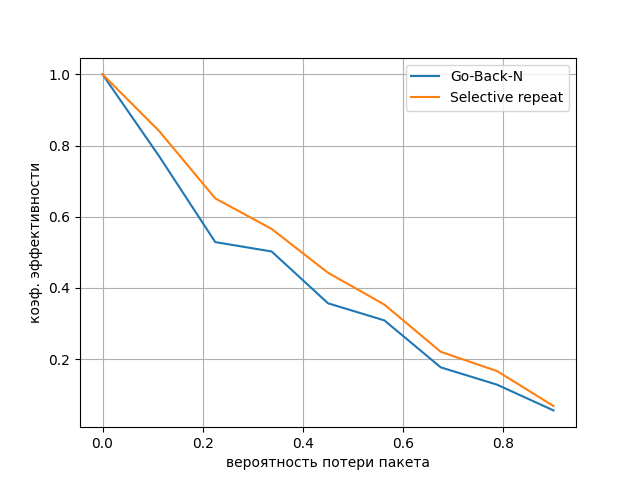
\includegraphics[width=\linewidth]{4.png} \\ Зависимость коэффициента
    эффективности от вероятности потери пакета при $w=3$}
\end{minipage}
\hfill
\begin{minipage}[h]{0.5\linewidth}
\center{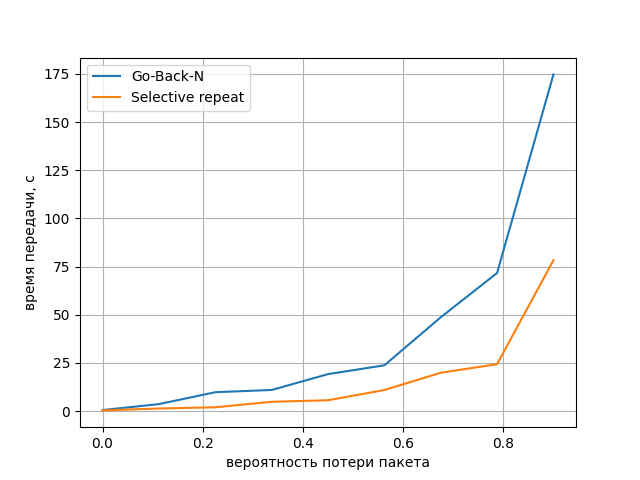
\includegraphics[width=\linewidth]{1.png} \\ Зависимость времени
    передачи от вероятности потери пакета при $w=3$}
\end{minipage}
\end{figure} 

\newpage

\subsection{Зависитость от размера окна}

\begin{table}[ht!]
    \begin{center}
        \caption{Зависимость эффективности протоколов от размера
        окна при $p=0.2$}\label{tab:2}
        \begin{tabular}{|c|c|c|c|c|}
        \hline
        w & \multicolumn{2}{|c|}{Go-Back-N} & \multicolumn{2}{|c|}{Selective repeat}\\
        \hline
          & t & k & t & k \\ 
        \hline
        2	 & 7.14  & 0.77    & 6.20  & 0.73   \\ \hline
        3	 & 6.08  & 0.65    & 1.97  & 0.74   \\ \hline
        4	 & 5.30  & 0.58    & 1.67  & 0.68   \\ \hline
        5	 & 4.63  & 0.55    & 2.23  & 0.65   \\ \hline
        6	 & 6.03  & 0.42    & 1.79  & 0.55   \\ \hline
        7	 & 3.50  & 0.51    & 1.16  & 0.64   \\ \hline
        8	 & 5.15  & 0.38    & 1.14  & 0.51   \\ \hline
        9	 & 5.35  & 0.35    & 1.33  & 0.48   \\ \hline
        10	 & 3.86  & 0.41    & 1.51  & 0.53   \\ \hline
        \end{tabular}
    \end{center}
\end{table}

\begin{figure}[ht!]
\begin{minipage}[h]{0.5\linewidth}
\center{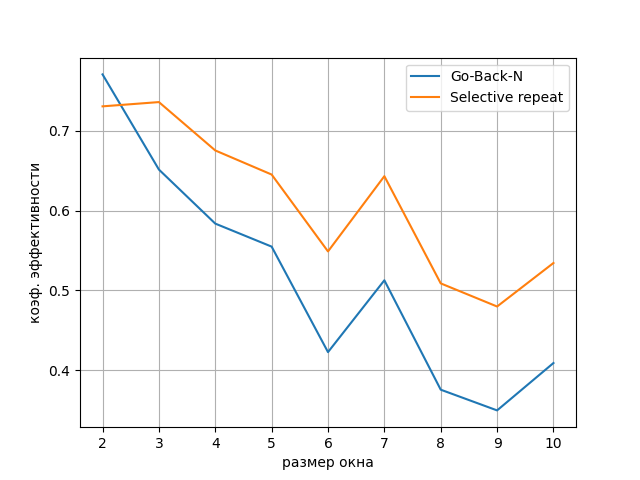
\includegraphics[width=\linewidth]{3.png} \\ Зависимость коэффициента
    эффективности от размера окна при $p=0.2$}
\end{minipage}
\hfill
\begin{minipage}[h]{0.5\linewidth}
\center{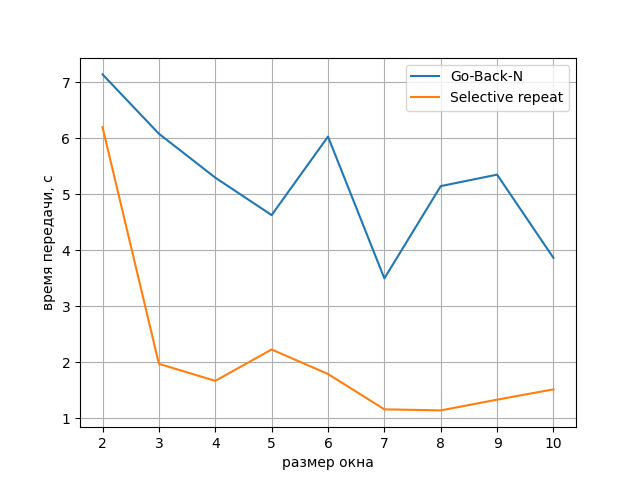
\includegraphics[width=\linewidth]{2.png} \\ Зависимость времени
    передачи от размера окна при $p=0.2$}
\end{minipage}
\end{figure} 

\section{Результаты}

По рассмотренным выше зависимостям можно сделать следующие выводы:

\begin{itemize}
    \item При малых вероятностях потери пакета эффективность протоколов 
        практически не отличается. Далее протокол \textit{Go-Back-N} все
        значительнее проигрывает протоколу \textit{Selective repeat}
    \item Зависимость от размера окна менее явная. Можно заметить, что для
        протокола \textit{Selective repeat} эффективность улучшается с
        увеличением окна. Протокол \textit{Go-Back-N} ведет себя более
        хаотично, но общая тенденция аналогична.
\end{itemize}

\end{document}
